\chapter{Least Squares method}

As we have seen in previous chapters the overall process to determine the location of the source is studying the correlation between the VTEC value and the solar-zenith angle (or source-zenith angle, speaking in general terms) for a possible location.

That is, for an IPP with a location and an associated VTEC value, given the location of a possible source, compute the cosine between them, and see that the closer the cosine to 1 (or 180º), the higher the VTEC value.

The idea that we wanted to test with this method was finding the location of the source by performing the inverse operation: having the VTEC, location of the IPP and correlation (1, assuming a near-linear correlation), obtaining the source's right ascension and declination.

\section{The equation system}

The source-zenith cosine between the source and the IPP was computed using the following equations:

\begin{equation} \label{eq:61}
unitVectorIPP =
\begin{bmatrix}
X' \\
Y' \\
Z'
\end{bmatrix}
=
\begin{bmatrix}
\cos\delta_{g} * \cos\alpha_{g} \\
\cos\delta_{g} * \sin\alpha_{g} \\
\sin\delta_{g}
\end{bmatrix}
\end{equation}

\begin{equation} \label{eq:62}
unitVectorSource =
\begin{bmatrix}
X \\
Y \\
Z
\end{bmatrix}
=
\begin{bmatrix}
\cos\delta_{s} * \cos\alpha_{s} \\
\cos\delta_{s} * \sin\alpha_{s} \\
\sin\delta_{s}
\end{bmatrix}
\end{equation}

\begin{equation} \label{eq:63}
\cos \chi = unitVectorIPP \cdot unitVectorSource
\end{equation}\\

Having the VTEC and source-zenith cosine, we could find the correlation of the two variables, expecting that the real source would yield a near-linear correlation.

Visually, we can see the relation between VTEC and the computed cosine in figure \ref{fig:solar-zenith-angle}, obtained in chapter 3 when studying the a specific case for the Sun.

\begin{figure}[!htb]
	\begin{centering}
		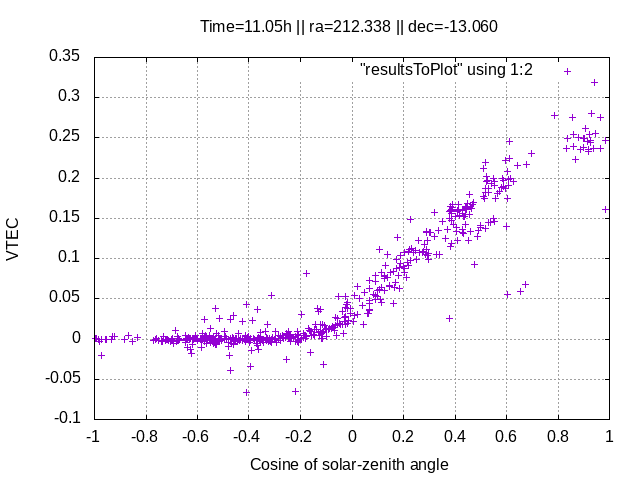
\includegraphics[width=0.5\linewidth]{images/ch4/resultSunTest.png}
		\caption{VTEC as a function of the solar-zenith angle's cosine}
		\label{fig:solar-zenith-angle}
	\end{centering}
\end{figure}

As we have previously seen for this case, there appears to be a linear relation starting around $\cos \chi = -0.1$ between the two studied parameters. Therefore, we could define this linear relation as a \textbf{straight line} ($y = mx + b$) by expressing the estimated VTEC value ($\Delta V$) as a function of the source-zenith cosine (\ref{eq:linearRelation}).

\begin{equation} \label{eq:linearRelation}
\Delta V = a\cos \chi + b
\end{equation}

Because the cosine is computed using the previous equations (\ref{eq:61}, \ref{eq:62}, \ref{eq:63}). It can be expressed as follows:

\begin{equation} \label{eq:cosine}
\cos \chi = XX' + YY' + ZZ'
\end{equation}

Where $X'$, $Y'$, $Z'$ are the components of the IPP's unit vector obtained from equation \ref{eq:61}, and $X$, $Y$, $Z$ are the unknowns of our equation: the components of the source's unit vector, which could be used to easily find the right ascension and declination of the source by using trigonometric operations.

However, finding the value of this unknowns is the difficult part of this method. Taking the cosine as \ref{eq:cosine} we can express the linear function as:

\begin{equation} \label{eq:substitute}
\Delta V = aXX' + aYY' + aZZ' + b
\end{equation}

Because $a$ and $b$ are unknowns as well as $X$, $Y$ and $Z$, we can group them as follows:

\begin{equation} \label{eq:newNames}
\Delta V = \alpha X' +  \beta Y' +  \gamma Z' + b
\end{equation}

Our aim now would be to solve the previous equation, but then we would need to obtain only the values of $X$, $Y$ and $Z$. We can see that:

\begin{equation} \label{eq:elTrucoDelAlmendruco}
\sqrt{\alpha^{2}+\beta^{2}+\gamma^{2}} = \sqrt{a^{2}(X^{2}+Y^{2}+Z^{2})} = \sqrt{a^{2}} = a
\end{equation}

Because $X$, $Y$ and $Z$ are the components of a unit vector\footnote{$\sqrt{(X^{2}+Y^{2}+Z^{2})} = 1$}. The previous allows us to, once we know the values of $\alpha$, $\beta$ and $\gamma$, obtain $X$, $Y$ and $Z$ by doing:

\begin{equation} \label{eq:iso}
\frac{\alpha}{\sqrt{\alpha^{2}+\beta^{2}+\gamma^{2}}} = \frac{\alpha}{a} = \frac{aX}{a} = X
\end{equation} \\

In our data we can find, for each IPP: $\Delta V$, $X'$, $Y'$, $Z'$ (because we have the right ascension and declination of the point).

For each of these IPPs, we have an equation of the form $\Delta V = \alpha X' +  \beta Y' +  \gamma Z' + b$ and, therefore, we have an overdetermined system of equations, with more equations (unknown, depends on the input data) than variables (four: $\alpha$, $\beta$, $\gamma$ and $b$)

Knowing how to obtain $X$, $Y$ and $Z$ from $\alpha$, $\beta$ and $\gamma$, we can now focus on solving the system of equations to obtain the latter unknowns .

Because we have an overdetermined system of equations, the solution can be approximated using the Least Squares approach. The system can be represented in matrix form $y = AX$ as follows:

\begin{equation} \label{eq:matrixSystem}
\begin{bmatrix}
\Delta V_{0} \\
\Delta V_{1} \\
. \\
. \\
. \\
\Delta V_{n}
\end{bmatrix}
=
\begin{bmatrix}
X'_{0} & Y'_{0} & Z'_{0} & 1 \\
X'_{1} & Y'_{1} & Z'_{1} & 1 \\
. & . & . & .\\
. & . & . & .\\
. & . & . & .\\
X'_{n} & Y'_{n} & Z'_{n} & 1 \\
\end{bmatrix}
\begin{bmatrix}
\alpha \\
\beta \\
\gamma \\
b \\
\end{bmatrix}
\end{equation}

This way, X can be obtained by means of the least squares estimate equation:

\begin{equation}
	X = (A^{T}A)^{-1}A^{T}y
\end{equation}

\section{Pseudocode}

\section{Implementation}

When

One of the main advantages of this method over the others is that we don't need to compute the correlation, that it is, discard outliers. (o si????)
